\documentclass[11 pt, twocolumn]{article}

\usepackage{hyperref}
\usepackage{titling}
\usepackage{amsmath,amssymb}
\usepackage{algorithm}
\usepackage[noend]{algpseudocode}
\usepackage[margin=0.8in]{geometry}
\usepackage{graphicx}
\usepackage{color}
\usepackage{enumitem}
\setlist[enumerate]{label*=\arabic*.}

\makeatletter
\def\BState{\State\hskip-\ALG@thistlm}
\makeatother

\setlength{\droptitle}{-5em}
\setlength{\columnsep}{2em}

\title{\textbf{GPU Monitoring tool for Reinforcement Learning algorithms}\\\Large CS236605 - Deep Learning, Computer Science Department\\Technion, Israel Institute of technology}

\author{Ira Gorodovskaya, Alexey Tusov}
\date{Spring 2019}

\newcommand{\todo}[1]{{\color{red} TODO: {#1}}}
\newcommand{\algspace}{\hspace{\algorithmicindent}}

\begin{document}
\maketitle
\section{Abstract}
Graphics Processing Units (GPUs) can significantly accelerate the training process for many deep learning models. Training deep learning models involves compute-intensive matrix multiplication and other operations that can take advantage of a GPU's massively parallel architecture.

However in practice, average GPU utilization for deep learning jobs tends to be surprisingly low, mainly because of common made algorithms and without customization for used hardware accelerators.

In this paper, we present a practical method for monitoring GPU metrics for the Arcade Learning Environment (ALE) and use it to benchmark GPU utilization among different Reinforcement Learning algorithms and try to find dependence between learning performances and GPU utilization.


\section{Introduction}
We started our project by benchmarking Evolution Strategies (ES) algorithms beside reinforcement learning (RL) algorithms, trying to understand what can cause difference in performances, main and the significant difference we pointed was massive parallel execution in ES algorithms meanwhile RL algorithms can be parallel in some cases but in many scales less parallel then ES. This cause us to think about the accelerators utilization in learning algorithms.


Researches in reinforcement learning (RL) have relied heavily on empirical evaluation, making experiment turnaround time a key limiting factor. Despite this critical bottleneck, many reference implementations do not fulfill
the potential of modern computers for throughput.
Efforts to parallelize and accelerate deep RL algorithms have been underway for several years. Recently, (Horgan et al., 2018\cite{horgan2018distributed}) showed that a distributed, prioritized replay buffer can support faster
learning while using hundreds of CPU cores for simulation and a single GPU for training. The same work used increased batch sizes, with a brief study of the effect of
learning rate.


Based on GPU's architecture we assume that serial RL algorithms may not utilize all available computing power provided by the GPU. And we want to understand if better GPU utilization may cause better learning performances.
In this work, we provide our implementation for GPU runtime monitoring, this tool could help to improve leverage by maximize performance of multiple CPUs and single GPU system (we made also a compatibility to support multi GPU monitoring), in purpose to gain significant improvement in efficiency, scale of hardware utilization and hence in learning speed.


\section{Methods}
\subsection{GPU architecture}
Execution in GPUs made by calling kernel methods from user space in CPU's level, each user process can call multiple GPU's kernels in synchronic modes and asynhronic modes, multiplying user processes means multiplying GPU's concurrent executed kernels, each kernel executed in at least one Thread Block (TB) and all TBs executed in one Streaming Multiprocessor (SM), each 32 threads in one TB grouped in Wrap and executed in parallel command level context. GPU's architecture supports multiple number of SMs and they all shares same global GPU memory, user's code in CPU level copies memory from CPU's global memory to GPU's global memory.
Data copy could be done by DMA transfer, which requires pinned memory in CPU's global memory and CPU's low memory availability in large parallel executions could be a bottle neck for such mechanism. In addition, data may be transferred using unified memory, which requires additional page management and may cause and additional overhead.
\begin{figure}
\centering
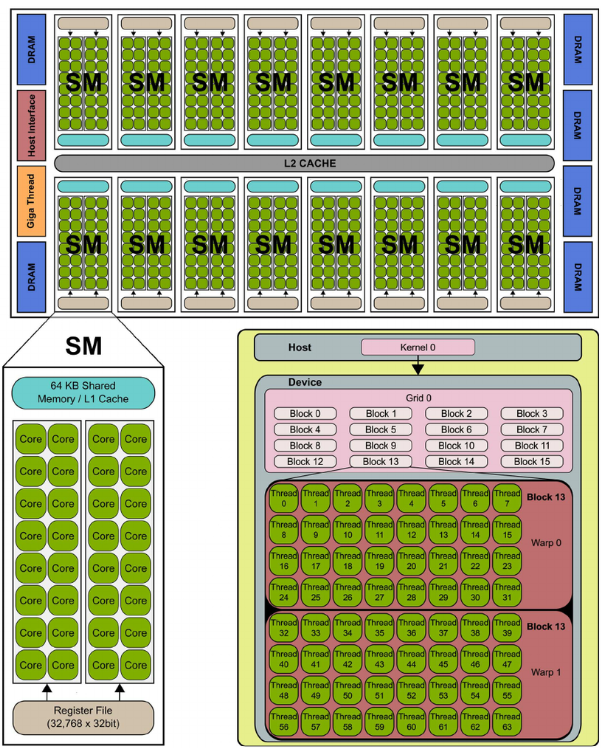
\includegraphics[width=0.93\columnwidth]{gpu_arch.png}
\caption{GPU architecture}
\vspace*{2pt}
\end{figure}

\subsection{RL algorithms}
Provide brief introduction
\subsection{Non parallel RL algorithms}
Provide brief introduction for DQN, figures could be great
\subsection{Parallel RL algorithms}
Provide brief introduction for A2C, figures could be great
\subsection{Data for evaluation}
For evaluation we prepared monitoring implementation of A2C, DQN, DDQN, Dueling DQN and Rainbow algorithms for Atari games learning, due to technical limitations we choose to use DQN and A2C (maybe also rainbow?) algorithms to learn playing Atari game Pong.

\section{Implementation and Experiments}
\subsection{GPUMonitor and GPUMonitorWrapper}
[ADD LINK TO OUT GITHUB]


\textbf{GPUMonitor} is the main class for communication with GPUs and providing requested runtime information using \textbf{py3nvml} package, this class we used as reference from 
torchlearning repository [ADD REFERENCE].
Supported GPU's real time information obtained: 
\begin{enumerate}
\item Device name
\item Device memory
\begin{enumerate}
\item Total available memory [Mb]
\item Used memory [Mb]
\item Free memory [Mb]
\item List of used memory by different processes 
\end{enumerate}
\item Temperature [Celsius]
\item Power
\begin{enumerate}
\item Used power [W]
\item Power limitation [W]
\end{enumerate}
\item Fan speed [Percent]
\item Utilization
\begin{enumerate}
\item GPU utilization [Percent]
\item GPU memory utilization [Percent]
\end{enumerate}
\end{enumerate}


\textbf{GPUMonitorWrapper} is a wrapper class for RL environments, this class inherits from Wrapper class and could be added to model's wrappers hierarchy. It's supports logging directly to ".csv" log file every episode using \textbf{ResultWriter} class. \textbf{GPUMonitorWrapper} is our implementation and R\textbf{esultWriter} class implemented by use with reference to Monitor class from bench package.

\subsection{RL agents}
We used as reference DeepRL-Tutorials repository [ADD REFERENCE] for A2C, DQN, DDQN, Dueling DQN and Reinbow implementations for our agents implementation and experiments.

\subsection{Experiments}
We used DQN and A2C (Maybe also Rainbow?) in the following scenarios: [ADD LIST]

\section{Results}
[List the results for all our experiments, add plots and explain what we can learn from it].


\section{References}

% I dont think it's relevant \ structured as they requested (https://vistalab-technion.github.io/cs236605/assignments/final-project)
% There may be relevant information, it may be copied to sections upper
%
%
%
%
%
%
%In a standard RL formulation as a Markov Decision Process, a learning agent aims to maximize the sum of discounted rewards experienced while interacting with an environment:
%$ R_t=\sum_{k=0}^\infty{\gamma^k r_{t+k}} $, where $r$ is the reward and $\gamma\leq 1$ the discount factor. The value of a state, $V(s_t)=\mathbb{E}\left[R_t|s_t\right]$, is defined as the expected return under a given policy.  The Q-value, $Q(s_t,a_t)=\mathbb{E}\left[R_t|s_t,a_t\right]$ is the same but first using action $a_t$ to advance.
%
%In policy gradient methods, the policy is directly parameterized as a distribution over actions, as $\pi(a|s;\theta)$. The \textbf{Advantage Actor-Critic} algorithm learns to estimate state values $V(s;\theta)$, and iteratively optimizes the policy on fresh environment experience using gradient steps as $\mathbb{E}\left[\nabla_\theta\log\pi(a_t|s_t;\theta)A_t\right]$, where $A(s,a)=Q(s,a)-V(s)$ is the advantage, estimated as $R_t - V(s_t)$.
%
%Q-value learning methods instead parameterize the Q-function $Q(s,a;\theta)$, which in \textbf{DQN} is regressed against an objective as: $\mathbb{E}[\left(y_i-Q(a_i|s_i;\theta)\right)^2]$, where $y_i$ is the data-estimated Q-value given by $y_i=r_i + \gamma \max_a Q(a|s_{i+1};\theta^-)$.  The target network $\theta^-$ is periodically copied from $\theta$.  Training data is selected randomly from a replay buffer of recent experiences, each to be used multiple times. The use of distributional learning was combined with five other enhancements under the name \textbf{Rainbow}: Double-DQN, Dueling Networks, Prioritized Replay, n-step learning, and NoisyNets.
%
%
%\section{Problem Description}
%
%\subsection{Main Objective}
%
%
%
%\subsection{Implementation}
%
%
%
%\section{Experiments}
%Common benchmarks for general RL algorithms are Atari games in the Arcade Learning Environment (ALE) for discrete control, and simulated robots using the MuJoCo physics engine in OpenAI
%Gym for continuous control.
%
%The Arcade Learning Environment (ALE) (Bellemare et al., 2013; Machado et al., 2017) is a framework composed of Atari 2600 games to develop and evaluate AI agents. OpenAI Gym, at https://gym.openai.com, is a toolkit for the development of RL algorithms, consisting of environments, e.g., Atari games and simulated robots, and a site for the comparison and reproduction of results.
%Try to draw your attention to
%
%\subsection{Setup}
%
%\subsection{Results}
%
%\section{Conclusion}
%GPUs are getting faster and faster but it doesn’t matter if the training code doesn’t completely use them. The good news is that for most people training machine learning models there is still a lot of simple things to do that will significantly improve efficiency.
%
%
%\bibliography{Refs}
%\bibliographystyle{ieeetr}
\end{document}